%%%%%%%%%%%%%%%%%%%%%%%%%%%%%%%%%%%%%%%%%%%
%
% From a template maintained at https://github.com/jamesrobertlloyd/cbl-tikz-poster
%
% Code near the top should be fairly standard and not need to be changed
%  - except for the document class
% Code lower down is more likely to be customised
%
%%%%%%%%%%%%%%%%%%%%%%%%%%%%%%%%%%%%%%%%%%%


\documentclass[landscape,a1,final,a4resizeable]{include/a0poster}

%%% Packages %%%%%%%%%%%%%%%%%%%%%%%%%%%%%%%%%%%%%%%%%%%%%%%%%%%%%%%%%


\usepackage{multicol}
\setlength{\columnseprule}{0pt}
\def\columnseprulecolor{\color{white}}
% \usepackage[srgb]{xcolor}
\usepackage{morefloats}
\usepackage[pdftex]{graphicx}
\usepackage{rotating}
\usepackage{amsmath, amsthm, amssymb, bm}
\usepackage{array}
\usepackage{booktabs}
\usepackage{multirow}
\usepackage{hyperref}
\usepackage[margin=1.5cm]{geometry}
\usepackage[pan gram]{blindtext}
\usepackage{setspace}
\usepackage[dvipsnames]{xcolor}
\usepackage{mwhmacros}
\usepackage{include/picins}
\usepackage{tikz}
\usetikzlibrary{shapes.geometric,arrows,chains,matrix,positioning,scopes,calc}
\tikzstyle{mybox} = [draw=black, rectangle]
\usepackage{dsfont}
\input{include/jlposter.tex}
% \input{include/preamble.sty}

%%% Commands %%%%%%%%%%%%%%%%%%%%%%%%%%%%%%%%%%%%%%%%%%%%%%%%%%%%%%%%%

\newcommand{\myItem}{\item[\color{camLightBlue}$\bullet$]}
\newcommand{\col}[1]{{\color{camLightBlue}\textbf{#1}}}%{\fbox{#1}}
% \newcommand{\myBox}[1]{\fbox{#1}}%{#1}%
\newcommand{\myBox}[1]{#1}%
\newcommand{\elbo}{\mathcal{L}}
\newcommand{\entropy}{\mathbb{H}}
\newcommand{\kl}{\mathbb{K}\mathbb{L}}


\newcommand{\X}{\B X}
\newcommand{\bx}[1]{\B x_{#1}} 
\newcommand{\sumi}{\sum_{i=1}^N}
\newcommand{\param}{\scalebox{0.8}{\B\Theta\hspace{-0.31em}}}
\newcommand{\tparam}{\scalebox{0.8}{\tilde{\B\Theta}\hspace{-0.31em}}}
\newcommand{\post}{p( \param|\B z)}

\newcommand{\eqnn}[1]{\begin{align}{#1}\end{align}}
\newcommand{\eqn}[1]{\begin{align*}{#1}\end{align*}} 

\newcommand{\bb}[1]{\ensuremath{ \left( {#1} \right)}}
\newcommand{\BB}[1]{\ensuremath{\left[ {#1} \right]}} 

\newcommand{\B}[1]{\ensuremath{  \mathbf{#1} } }

%%% Color Definitions %%%%%%%%%%%%%%%%%%%%%%%%%%%%%%%%%%%%%%%%%%%%%%%%%%%%%%%%%
\definecolor{camBlue}{rgb}{.629,.757,.678}
\definecolor{camLightBlue}{rgb}{.416,.678,.894}
\definecolor{camDarkBlue}{rgb}{.208,.339,.447}
\definecolor{darkgreen}{rgb}{0,0.8,0}
\definecolor{darkblue}{rgb}{0,0.08,0.45}
\definecolor{blue}{rgb}{0,0,1}
%\definecolor{bordercol}{RGB}{40,40,40}
%\definecolor{bordercol}{RGB}{150,150,150}
\definecolor{bordercol}{RGB}{0,0,0}
%\definecolor{headercol1}{RGB}{186,215,230}
\definecolor{headercol1}{RGB}{200,200,200}
%\definecolor{headercol2}{RGB}{80,80,80}
\definecolor{headercol2}{RGB}{255,255,255}
%\definecolor{headerfontcol}{RGB}{0,0,255}
\definecolor{headerfontcol}{RGB}{0,0,0}
%\definecolor{boxcolor}{RGB}{186,215,230}
\definecolor{boxcolor}{RGB}{255,255,255}


%%% Eye Cacther %%%%%%%%%%%%%%%%%%%%%%%%%%%%%%%%%%%%%%%%%%%%%%%%%%%%%%%%%%%%%%%

\begin{document}
\begin{minipage}[t][0pt]{\linewidth}
\hspace{-6cm} 
%Align with edge of page, not margin
\vspace{-1.5cm}

\begin{tikzpicture}[overlay]
    \draw [fill=camLightBlue,draw=none] (0, 5) rectangle (100,-6.9);
    \draw [fill=camLightBlue,draw=none] (0, -56.7) rectangle (100,-100);
\end{tikzpicture}

{
\hspace{0.5cm}
\parbox{.2\textwidth}{
  % \vspace{-.5cm}
  \includegraphics[height=8cm]{badges/Utoronto_badge} \hspace{1cm}% 
  \vspace{-.5cm}\mbox{\vspace{-1cm}\includegraphics[height=6cm]{badges/cambridge_badge} \hspace{1cm}}
  }
\hspace{-2cm}
\parbox{.65\textwidth}{
  \vspace{0.5cm}%
  \begin{center}\color{white}
   \huge \textbf{Mapping Gaussian Processes to Bayesian Neural Networks}\vspace{3mm}\\
    \large Daniel Flam-Shepherd$^{\,1}$, James Requeima$^{\,2\,3}$, David Duvenaud$^{\,1}$\\
    \color{white}\large 
    $1$ University of Toronto, $2$ University of Cambridge, $3$ Invenia Labs
    \end{center}
  }%
\hspace{2cm}
\parbox{.05\textwidth}{  
  \begin{flushright}\vspace{-0.5cm}\includegraphics[height=6cm]{badges/inv_labs}\hfill% 
  \end{flushright}}
}%


%%%  Main Body %%%%%%%%%%%%%%%%%%%%%%%%%%%%%%%%%%%%%%%%%%%%%%%%%%%%%%%%%%%%%%%

\begin{poster}%
% Potentially add some space at the top of the poster
\vspace{0\baselineskip}%
\vspace*{0.7cm}%
\large%
\noindent%

\begin{multicols}{3}

%%% First Column %%%%%%%%%%%%%%%%%%%%%%%%%%%%%%%%%%%%%%%%%%%%%%%%%%%%%%%%%%%%%%%

\begin{minipage}[t][47.5cm][t]{.32\textwidth}

%\mysection{Drug and Material Design}{

%\col{\bf Goal}: find novel molecules that optimally fulfill various metrics: drugs, OLEDs, OPVs, etc.

%How to efficiently find new molecules with improved properties?

%% \begin{center}
%% 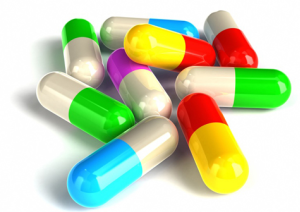
\includegraphics[width=0.275\textwidth]{motivation/pills.pdf}
%% \hspace{0.5cm}
%% 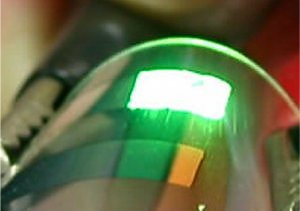
\includegraphics[width=0.275\textwidth]{motivation/oled.pdf}
%% \hspace{0.5cm}
%% 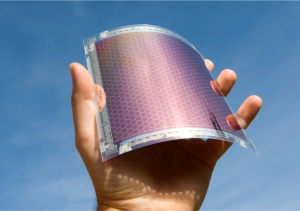
\includegraphics[width=0.275\textwidth]{motivation/opv.pdf} 
%% \end{center}

%\vspace{-.15cm}
%About $10^8$ compounds available in databases, but potential $10^{20} - 10^{60}$ new molecules! However,
%\begin{itemize}
%\item \textcolor{Peach}{\bf Evaluating molecular properties is slow/expensive}.
%\vspace{-.15cm}
%\item \textcolor{Peach}{\bf Chemical space is huge}.
%\end{itemize}
%{\bf Solution}: use \col{\bf Bayesian optimization} (BO) to accelerate the search.
%}

%\vspace{0.5cm}

\mysection{Priors in Function Space}{

\vspace{-1cm}
\begin{itemize}
  \item \col{\bf Baysian Neural Network Priors} are specified in parameter space. The implications of these priors in function space are hard to interpereate.
  \item How to we encorporate prior knowledge about function properties in our prior?
\end{itemize}
}
\vspace{0.5cm}


\mysection{Gaussian Processes}{
\col{Gaussian Processes} have a elegant mechanism for incorporating 
prior beliefs about the underlying function - the mean and covariance functions.\vspace{1cm}\\
\includegraphics[width=\textwidth]{figures/kernels.pdf}
Kernels can be combined using addition and multiplication to construct kernels with desired properties.\\
\includegraphics[width=\textwidth]{figures/kernels2.pdf}\\
}

\vspace{1cm}

% \mysection{}{
% The acquisition function in TS is a sample from the posterior.
% \begin{center}
% \includegraphics[width=0.625\textwidth]{figures/thompson_sampling/figure3.pdf}\\
% \end{center}  

% \textcolor{Peach}{\bf Conditioning to fantasies does not change posterior. 
% }
% }

\end{minipage}

%%% Second Column %%%%%%%%%%%%%%%%%%%%%%%%%%%%%%%%%%%%%%%%%%%%%%%%%%%%%%%%%%%%%%%
\hspace{0.25cm}
\begin{minipage}[t][47.5cm][t]{.32\textwidth}


%\vspace{1cm}

\mysection{Mapping the Prior}{We apprioximate the \col{KL divergence} between the Gaussian process $p_{\text{GP}}({\bm f})$ and the BNN prior over functions $p_{\text{BNN}}({\bm f}))$.
\begin{eqnarray*}
    \mathcal L_{p(\bm X)} (\bm \phi) & = &
    \E_{p(\bm X)}[\mathcal{KL}[p_{\text{BNN}}(\bm f(\bm X) |  \bm \phi ) \mid   p_{\text{GP}} (\bm f (\bm X) )]] \\
    & = & \E_{p(\bm X)}[-\mathcal{H} [p_{\text{BNN}} (\bm f (\bm X) |  \bm \phi ) ] \\
    && \,\,\,\,\,\,\,\,\,\,\,\,\, - \E_{p_{\text{BNN}} (\bm f  |  \bm \phi ) } [\log p_{\text{GP}} (\bm f (\bm X) ) ]    ]
\end{eqnarray*}

The second term in this expectation can be approximated using Monte Carlo. The entropy term can be approximated 
\begin{enumerate}
  \item  
\end{enumerate}


}


\end{minipage}


%%% Thirtd Column %%%%%%%%%%%%%%%%%%%%%%%%%%%%%%%%%%%%%%%%%%%%%%%%%%%%%%%%%%%%%%%
\hspace{0.5cm}
\begin{minipage}[t][14cm][t]{.3\textwidth}

%\vspace{1cm}


\mysection{Results: Bayesian Neural Networks}{
\includegraphics[width=\textwidth]{figures/results_thompson_sampling.pdf}

\col{\bf Data sets}:

\begin{itemize}
\item CEP: Harvard Clean Energy Project data, 2.3M molecules. 
\item One-dose: percentage cell growth relative to control, 27,000 molecules.
\item Malaria: drug concentration giving half max response, 19,000 molecules.
\end{itemize}

\col{\bf Batch sizes}: 500 (CEP) and 200 (Malaria and One-dose).
}

\vspace{1cm}


\mysection{Comparison with $\epsilon$-greedy sampling}{
\vspace{-.5cm}
\centering
Average rank and standard errors:\\
\includegraphics[width=0.4\textwidth]{figures/epsilon_table}

}

\vspace{1cm}

\mysection{Conclusions}{
We have proposed a batch BO method that 
\begin{itemize}
\item runs in a parallel and distributed manner.
\item can handle large batch sizes and large molecule libraries.
\item is comparable to non-scalable approaches (parallel EI) in small problems with GPs.
\item outperforms other alternative scalable approaches in large scale settings with Bayesian neural networks.
\end{itemize}
}
\end{minipage}

\end{multicols}
\end{poster}
\end{minipage}
\end{document}

